\documentclass[12pt]{article}
\usepackage[a4paper, hmargin={2.5cm, 2.5cm}, vmargin={2.5cm, 2.5cm}]{geometry}
\linespread{1.5}
\usepackage{eso-pic} % \AddToShipoutPicture
\usepackage{graphicx} % \includegraphics
\usepackage[utf8]{inputenc}
\usepackage[danish]{babel}
\usepackage[T1]{fontenc}
\usepackage{hyperref}
\usepackage{amsmath, amscd}
\usepackage{amsmath,amscd}
\usepackage{amssymb}
\usepackage{amsthm}
\usepackage{enumerate}
\usepackage{graphicx}
\usepackage{framed}
\usepackage{color}
\usepackage{listings}
\usepackage{float}
\usepackage{dirtree}
\lstset{
	frame=single,
	breaklines=true,
	postbreak=\raisebox{0ex}[0ex][0ex]{\ensuremath{\color{red}\hookrightarrow\space}}
}
\newcounter{nodeCdepth}
\newenvironment{nodeC}
{\ifnum\value{nodeCdepth}=0
    \gdef\listfordirtree{}%
    \let\item\nodeCitem
    \fi
    \stepcounter{nodeCdepth}}
{\addtocounter{nodeCdepth}{-1}%
    \ifnum\value{nodeCdepth}=0
    \expandafter\dirtree\expandafter{\listfordirtree}%
    \fi}
\newcommand{\nodeCitem}[1]{%
    \xdef\listfordirtree{%
        \unexpanded\expandafter{\listfordirtree}%
        .\thenodeCdepth\space\unexpanded{#1}. }%
}
%% Change `ku-farve` to `nat-farve` to use SCIENCE's old colors or
%% `natbio-farve` to use SCIENCE's new colors and logo.
\def \ColourPDF {../include/ku-farve}

%% Change `ku-en` to `nat-en` to use the `Faculty of Science` header
\def \TitlePDF {../include/ku-en}  % University of Copenhagen

\title{
  \vspace{3cm}
  \Huge{Eksamensrapport} \\
  \Large{Software Udvikling 2016 - Project-Stock}
	}

\author{
	\Large{Stefan Friis Tofte} - \textbf{jwr342} - \texttt{stefan.f.tofte@gmail.com}
	\and
	\Large{Mads Kronborg} - \textbf{xlq446} - \texttt{kronborg96@gmail.com}
	\and
	\Large{Lasse Halberg Haarbye} - \textbf{lpt113} - \texttt{ninjalf2@gmail.com}
	\and
	\Large{Christian E.N. Hansen} - \textbf{vmk541} - \texttt{cralle@outlook.com}
}


\begin{document}


\AddToShipoutPicture*{\put(0,0){\includegraphics*[viewport=0 0 700 600]{\ColourPDF}}}
\AddToShipoutPicture*{\put(0,602){\includegraphics*[viewport=0 600 700 1600]{\ColourPDF}}}

\AddToShipoutPicture*{\put(0,0){\includegraphics*{\TitlePDF}}}

\clearpage\maketitle
\thispagestyle{empty}

\newpage
\tableofcontents
\newpage

\section{Indledning}
\label{sec:indledning}
% Christian

\section{Problembeskrivelse}
\label{sec:problem}
Vores projekt er udviklet som en løsning på, den tildels besværlige proces, som det kan være at tilmelde sig bachelorprojekter. Jyrki som er medansvarlig for bachelorprojekterne, ønskede en mindre manuel løsning en den forværende. Det største problem i den tidligere løsning, opstod når elever skulle gå fra professor til professor og få afslag. Yderligere har problemer som den nye reform, gjort det endnu vigtigere at få en hurtigere og smartere metode. \\
Vi har derfor lavet en side, som ved automatisk scraping af informationer fra diku's hjemmeside, kan præsentere en up-to-date visning af de forskellige ledige projekter og vejledere, samt deres arbejdsbyrd. Opsumeret har vi altså fået implementeret alle ''Quality requirements''. \\
Vi kunne til gengæld ikke opfylde alle de funktionelle krav, da et punkt som f.eks. "There should be a mechanism to check the quality of industrial projects" er for subjektivt og vi hverken har erfaring eller viden omkring dette. \\
Ligeledes har vi også valgt ikke at implementere en løsning, hvor studerende kan lave et "ønske-opslag" om uaktuelle emner, i håb om at nogle vejledere vil lave et projekt om det.


\section{Krav}
\label{sec:krav}
I forløbets start opstillede vi nogle \textit{use cases}, for at imødekomme de krav vores \textit{product owner} havde til det produkt vi skulle udvikle. \\
Vi foretog en løs priotering af produktets \textit{use cases}. Vi vurderede, hvad der var kernefunktionaliteter, og hvad der var \textit{'nice-to-have'}-funktionaliteter.

\subsection*{\textit{Use cases}}

\subsubsection{Kernefunktionaliteter}
\label{sec:corefuncs}
\begin{enumerate}
	\item Det skal være muligt at se et katalog over projekter.
	\item Systemet skal kunne præsentere \textit{up-to-date} oplysninger om potentielle vejledere, herunder:
	\begin{itemize}
		\item Tidligere projekter.
		\item Forskningspublikationer.
		\item Kontaktoplysninger.
	\end{itemize}
	\item Personer, der optræder på siden, skal kunne verificeres, hvis de eksempelvis ønsker at tilføje projekter eller foretage rettelser.
\end{enumerate}

\subsubsection*{\textit{'Nice-to-have'}-funktionaliteter}
\label{sec:nicefuncs}
\begin{enumerate}
  \item Systemet skal kunne vise projekter knyttet til specifikke \textit{keywords}.

  \item Systemet skal vise en status på en vejleders arbejdsbyrde \textit{up-to-date} (hvad der præcist menes med dette, skal yderlige specificeres).
  \item En vejleder eller en person knyttet til en \textit{business-club}, skal kunne tilføje et projekt til projektkataloget.

	\item Systemet skal kunne filtrere vejledere i forhold til \textit{keyswords} i forskningspublikationer (titler).
\end{enumerate}


\section{Design}
\label{sec:design}
% Lasse
\subsection{Struktur}
Et Django-projekt har en struktur der ser således ud:\\
\begin{nodeC}
    \item{project\_stock}
    \begin{nodeC}
        \item{manage.py}
        \item{project\_stock}
        \begin{nodeC}
            \item{\_\_init\_\_py}
            \item{apps.py}
            \item{models.py}
            \item{settings.py}
            \item{tests.py}
            \item{urls.py}
            \item{views.py}
            \item{wsgi}
        \end{nodeC}
    \end{nodeC}
\end{nodeC}~\\
Nogle af disse filer følger med når man starter et projekt fra bunden, bl.a. \_\_init\_\_.py, settings.py, urls.py og wsgi.py\\
% Forklaring følger
\\
Vores specifikke struktur kan findes i bilag under ...

\subsection{Modularitet}
Django er bygget op således at alle . Altså kan man tilføje/fjerne \texttt{models.py} for at tilføje/fjerne projektets databasestruktur. Ligeledes kan man tilføje/fjerne \texttt{tests.py} afhængigt af om man vil have tests. Alternativt kan man lave en undermappe der hedder tests og placere sine \texttt{test\_*.py} filer her. Dette er en funktion indbygget i Pythons \texttt{unittest} modul, som automatisk leder i denne mappe efter navne der starter med "test".
Dette har vi gjort for at dele vores unit tests op og dermed gøre dem lettere overskuelige. F.eks. har vi både en fil til at teste vores models og en til at teste vores views, \texttt{test\_models.py} og \texttt{test\_views.py}.
% Forklar views og models tidligere? i introduktion måske?

\subsection{Scraper(e)}
Vi har en funktionel scraper, der kan gemme information fra diku.dk/Ansatte, og alle underlinks for alle ansatte på siden.\\

\begin{figure}[H]
    \centering
    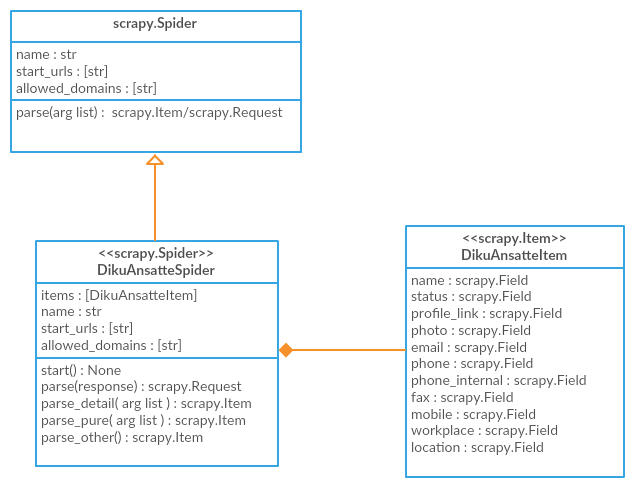
\includegraphics[scale=0.5]{scraper_class_diagram.png}
    \caption{Scraper klassediagram}
    \label{fig:scraper_class_diagram}
\end{figure}

\subsection{Frontend}
Under designet af vores frontend har der ikke været fokus på det æstætiske eller brugervenlighe, men i stedet på hvor meget information vi kan distribuere til studerende som muligt. Vi påstår ikke at et flot og brugervenligt design ikke er vigtigt, men vi ville helst opfylde så mange krav så muligt, og æstætik var ikke en prioritet.\\
\\
Herunder har vi de mest essentielle sider i vore webapplikation.

\subsubsection{Projekter og vejledere}
\begin{figure}[H]
    \centering
    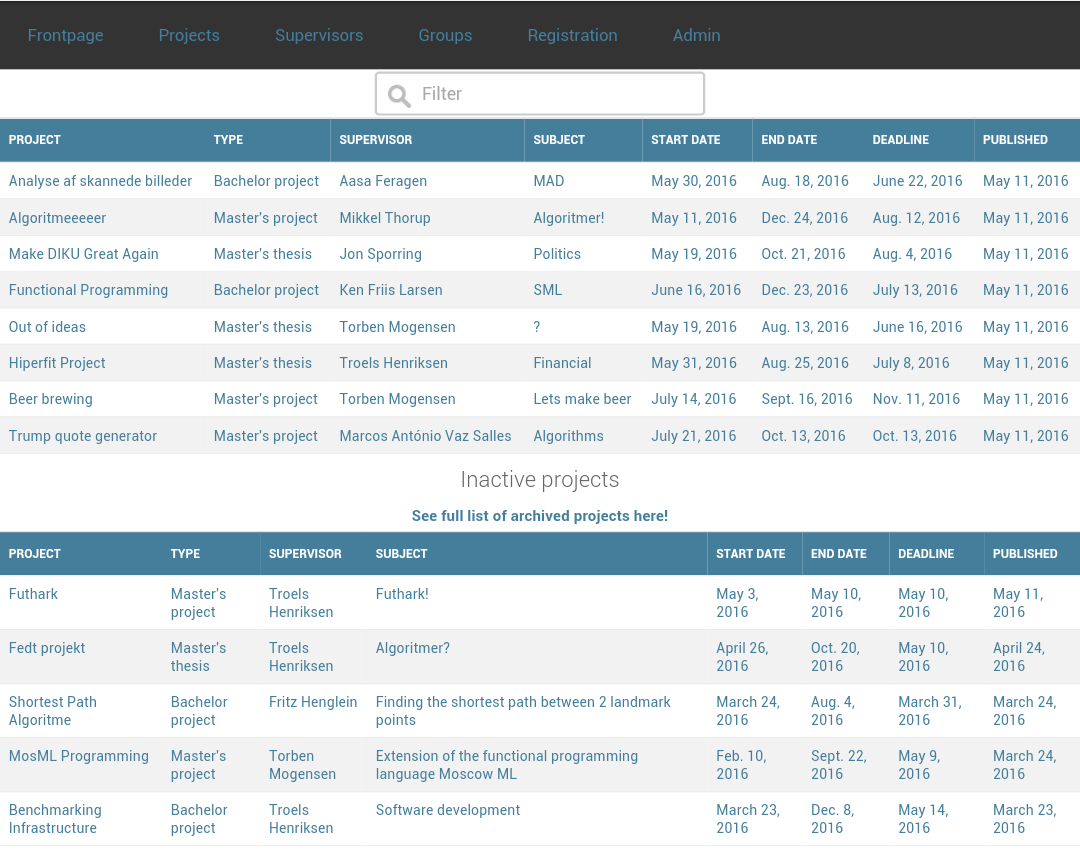
\includegraphics[scale=0.33]{frontend_projects.png}
    \caption{Oversigten over projekter på siden}
    \label{fig:frontend_projects}
\end{figure}
\begin{figure}[H]
    \centering
    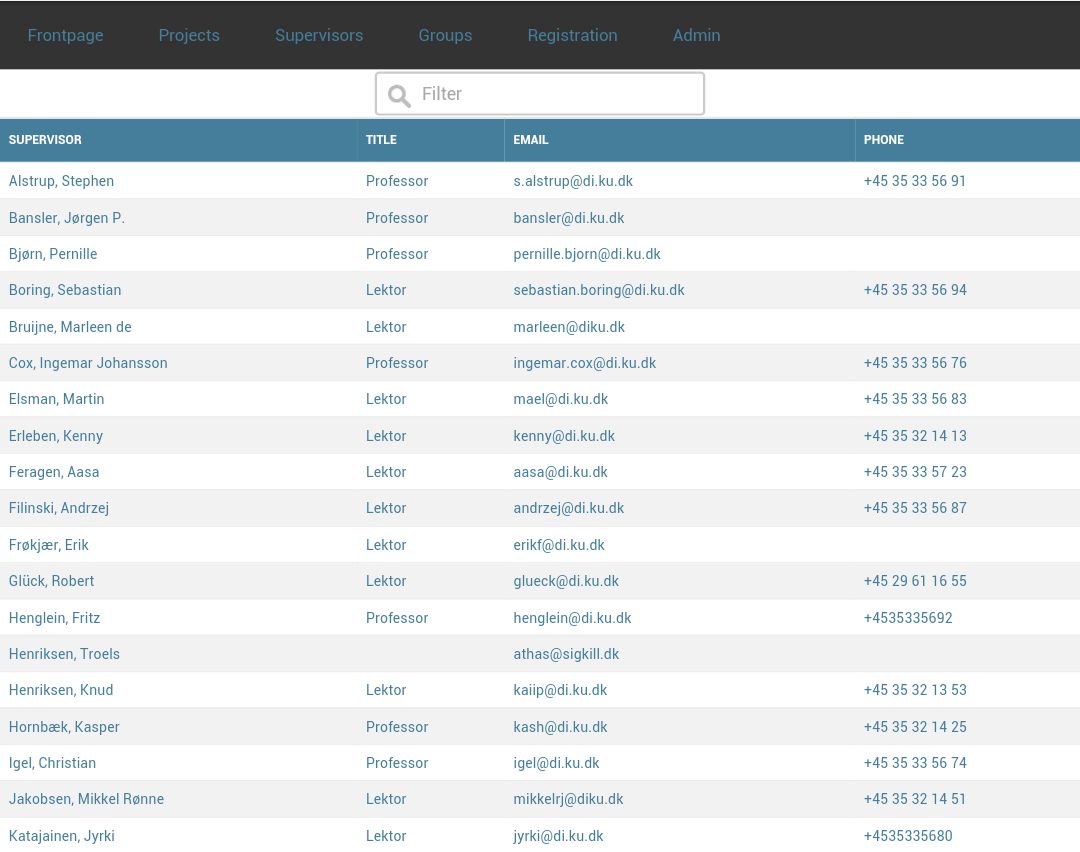
\includegraphics[scale=0.33]{frontend_supervisors.png}
    \caption{Oversigten over vejledere på siden (ikke alle vejledere kan ses på billedet)}
    \label{fig:frontend_supervisors}
\end{figure}
~\\
\hyperref[fig:frontend_projects]{Figur \ref*{fig:frontend_projects}} og \hyperref[fig:frontend_supervisors]{figur \ref*{fig:frontend_supervisors}} viser de to vigtigste sider i vores webapplikation. Disse to sider viser information omkring projekter og vejledere, og opfylder dermed henholdsvis krav 1 og 2 fra \hyperref[sec:corefuncs]{\ref*{sec:corefuncs} \nameref*{sec:corefuncs}}.\\

\subsubsection{Groups}
\begin{figure}[H]
    \centering
    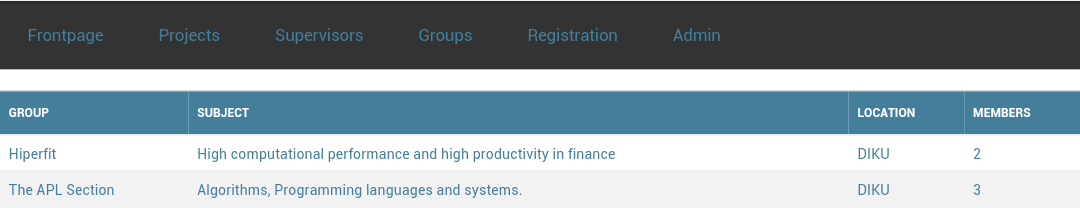
\includegraphics[scale=0.33]{frontend_groups.png}
    \caption{Oversigten over grupper på siden}
    \label{fig:frontend_groups}
\end{figure}
Her kan studerende se en oversigt over grupper med vejledere inden for et specifikt felt og dermed finde adskillige vejledere inden for feltet som den studerende interesserer sig for.
Denne side opfylder krav 1 under \hyperref[sec:nicefuncs]{\ref*{sec:nicefuncs} \nameref*{sec:nicefuncs}}.

\subsubsection{Registrering}
Her kan en vejleder registrere sig på siden, men kun hvis vejlederen allerede står som vejleder på siden, enten indhentet vha. scraperen eller indtastet manuelt af en "superuser".\\
% forklar superuser
Siden er ikke helt funktionel, da den ikke rigtigt gør noget, men dette ville ikke kræve meget ekstra arbejde,.
Denne side ville opfylde krav 3 fra \hyperref[sec:corefuncs]{\ref*{sec:corefuncs} \nameref*{sec:corefuncs}}, hvis den havde været færdigimplementeret.\\

\subsubsection{Adminpanel}

\newpage
\section{Afprøvning}
\label{sec:afproevning}
Til afprøvning og test af projektet gjorde vi os nogle forskellige overvejelser, vi var bl.a. i tvivl om hvorvidt vi
skulle anvende Fitnesse eller robot frameworket. Vi endte med at bruge robot til at skrive automatiske acceptancetests.
Disse tests er yderligere beskrevet i Bilag E.\\
Vi har valgt ikke at sikre applikationens opfyldelse af krav ved tests. Det har vi gjort grundet, at vi prioriterede
færdigudvikling af projektet over hvad vi vil mene er overflødig test. Her menes der, at vi kan se og ved at hjemmesiden
opfylder de stillede krav fra det tidligere krav-afsnit. Det ved vi fordi, vi har brugt og manuelt bevæget os rundt på
hjemmesiden, løbende har opdaget fejl og mangler og har fået dem implementeret. \\
Til fremtidig brug er vores acceptance-tests skrevet således at selvom der skulle opstå ændringer på hjemmesiden, kan vi
nemt bruge dem igen. Det kan vi fordi de tilgår elementer i den tabel, som hjemmesiden repræsenterer information i, i
stedet for at tilgå de specifikke elementer cellerne indeholder. For testen er det altså ligegyldigt hvad der står i
tabellen, bare siden har samme struktur. Skulle selve strukturen af sitet dog ændres, kan vi forholdsvis nemt omskrive
testene til at tilgå elementer på en ny måde, da det blot er kodedelen som beskriver hvilket element der skal tilgås, som
skal omskrives. \\ 
Da vores tests, som beskrevet ovenfor, er forholdsvis automatiske og agile, kan vi nemt anvende dem når vi tilføjer ting
til sitet, eller ændrer på de ting som i forvejen er tilstede. Det har givet mulighed for ubesværet at teste, mens vi har
arbejdet på projektet. \\
Selvom vi bruger django, som er et færdiggjort og stort framework, har vi valgt at unit-teste dele af projektet, for at
sikre fejlbarheden så vidt som muligt. Django-funktionerne har vi i grove træk testet ved at opsætte to scenarier for de
forskellige framework funktioner, ét scenarie som får forkerte specifikationer og ét scenarie som får de korrekte. Således
kan vi se om de fejler eller kører som ønsket og forventet. Disse tests er også yderligere beskrevet i Bilag E. 

\section{Udviklingsmiljø}
\label{sec:udvikling}
Vi vil i dette afsnit beskrive vores opsætning af versionsstyring, og hvordan vi har opbygget vores struktur for projektet. Endvidere hvilke værktøjer vi har brugt og hvordan vi har brugt dem.

\subsection{Opsætning og struktur}
Vi har brugt versionsstyringsværktøjet \textit{git} til dette projekt, git holder styr på de filer du har lagt ind i dit \textit{repository}, filernes ændringer og sørger for at man let kan dele filerne imellem flere udviklere. Et repository er i en software udviklings sammenhæng en mappe hvori man gemmer alle de filer, som tilsammen udgør et projekt. \\
Vores repository er struktureret sådan, at vi gemmer vores rapporter og andet i en separet mappe, fra selve vores produkt, dog stadig i samme repository. På denne måde kan vi også bruge versionsstyring til at skrive sammen.

\begin{figure}[H]
	\centering
	\includegraphics[scale=0.55]{repostruct.png}
	 \caption{Abstrakt struktur af vores repository}
	 \label{fig:repostruct}
\end{figure}
~\\
Figur \ref{fig:repostruct} viser strukturen af vores repository, vi har valgt at lave figuren abstrakt og undladt visse mapper, dels fordi vi skriver i frameworket \textit{Django}, som har en del filer og mapper som skal være der, men som vi ikke rigtig selv har brugt særligt meget. Filen \textit{manage.py} er vigtig eftersom, det er den fil som styrer selve hjemmesiden, det er med den fil man starter en webserver, opdaterer ens database og andet. Hjemmesiden indeholder en masse Django specifikke filer, sådan som et database schema, templates til selve hjemmesiden og meget andet.

\subsection{Git}
Vi har igennem projektet fået arbejdet meget med git, og vi har alle lært en del omkring git. I starten af projektet fik vi mange merge-conflicts hvilket betyder, at git ikke ved hvilke ændringer i hvilke filer er de rigtige ændringer, hvilket sker hvis der er blevet ændret i samme fil ved samme sted. Vi undersøgte problemet, og fandt frem til nogle git-opsætninger som hjalp med at undgå disse merge-conflicts. Derudover har vi skrevet tips til at bruge git ind i vores \textit{README.md}, som beskriver små tips til hvordan man kan benytte git mere effektivt. \\ \\
Vi har brugt vores README.md rigtig meget igennem projektet til at dele tanker, tips og bare generelle informationer specifikt til projektet. Dette kan være alt fra, hvilke hjemmesider vi kan scrape, og hvordan man kan scrape det, til at dele youtube videoer der beskriver Django.

\subsection{Udviklingsmiljø}
Vi har til projektet besluttet ikke at bruge et specifikt IDE til at udvikle i. Grunden til dette er, at vi alle har forskellige præferencer og arbejder bedst på forskellige måder. Nogen af os vil gerne have en simpel IDE (\textit{Integrated Development Environments}, Text editor), såsom Emacs, som ikke kan så meget fra starten af, men hvor man kan tilføje funktioner og værktøjer for at tilpasse IDEen, og andre fra gruppen ville hellere have en større IDE, såsom Atom, som fra start kan en hel del mere. \\ \\
Vi besluttede os for at vi hver især arbejder mere effektivt og bedre, hvis vi udvikler i det miljø der passer os bedst indviduelt. Det vil sige, at nogle medlemmerne af vores gruppe, selv har stået for at kunne afprøve programmet, lave refaktorering og afvikling af hjemmesiden. At kunne gøre brug af værktøjer til refaktorering har ikke været et stort problem til vores projekt, da som tidligere nævnt er Django meget specifik, og klasser, funktioner og andet skal se ud på en meget bestemt måde. Det samme gælder for kode kreation, som bliver håndteret af manage.py.

\section{Diskussion og reflektion} % Alle
\label{sec:diskussion}

\subsection{Testing}
\subsubsection{\textit{Test-first} og \textit{TDD}}
I vores arbejde med projektet, har vi ikke benyttet princippet \textit{test-first}, der b.la. kendes fra metodologien \textit{Extreme Programming (XP)}.
Vi har senere erfaret, at det kunne have været nyttigt, i visse tilfælde, havde vi benyttet en \textit{test-first} tilgang. Dels fordi det ville være nemmere at \textit{unit teste} vores kode, og dels fordi det formentlig havde ført til at vi havde skrevet kode, der var mere afkoblet. \\
Vores begrundelse for ikke benytte \textit{test-first}, var at det var svært at forene med \textit{Django frameworkets} faste krav for, hvordan koden skal struktureres. \\
Derimod kunne vi godt have have benyttet en \textit{test-first} tilgang til vores \textit{web scraper}. Koden for vores \textit{scraper} findes i filen \texttt{dikuspider.py}.

\subsection{\textit{Web scraper}}
Den \textit{web scraper} vi har udviklet, er designet til at høste data fra siden \url{http://diku.dk/ansatte}, samt profilsiderne for Datalogisk Instituts ansatte. Der linkes til disse profilsider fra \url{http://diku.dk/ansatte}.\\
Vi har vurderet, at det ville være svært og formentlig unødigvendigt at designe en abstrakt \textit{scraper}, som ville være i stand til at høste data fra mange forskellige websteder. At ekstrahere data fra et specifikt websted, afhænger i høj grad af, hvordan dette websted er opbygget. Er den information man er interesseret i, f.eks. placeret i  HTML-tabeller, skal man vide hvilke \textit{id tags} man skal ledes efter. Ligeledes skal man vide, hvordan denne information er formatteret. \\
Da vi ikke har fundet andre websteder, hvor man kan høste information om de ansatte, vurderede vi at ikke ville være i overenstemmelse med agile tankegang at prøve at designe en abstrakt \textit{scraper}.

\section{Videreudvikling}
\label{sec:udvikling}
Vi vil diskutere hvilke krav som vi ikke nåede at implementere, men som vi gerne ville have lavet givet mere tid. Dette kan ses som en liste over brugs-scenarier eller \textit{use cases}, som et hold af udvikler skulle modtage, hvis de overtog vores projekt efter afslutningen af vores projekt. \\ \\
\begin{itemize}
\item Verifikation og oprettelse af vejledere i systemet. Vi nåede ikke at lave et færdigt system til at lade vejledere registere sig i vores system, så de selv kan ligge projekter op på hjemmesiden.
\item Man skal kunne se en liste over publikationer hos en vejleder, og en vejleder skal kunne ligge publikationer ind på sin side.
\end{itemize}

\section{Konklusion}
\label{sec:konklusion}
% Christian

\begin{thebibliography}{9}

\bibitem{agile}
	Martin, R.C., Martin, M.,
	\emph{Agile Principles, Patterns, and practices in C\#},
	Upper saddle river, NJ, Prentice Hall,
	2007

\bibitem{cc}
	Steve McConnell,
	\emph{Code Complete},
	2nd edition,
	2004.

\end{thebibliography}


\section{Bilag}
\label{sec:bilag}

\subsection{Bilag A}
\label{sec:bilagA}
\begin{center}
	\begin{tabular}{|p{0.05\textwidth}|p{0.5\textwidth}|p{0.45\textwidth}|}
		\hline
	\textbf{D\#} & \textbf{Færdigimplementerede \textit{use cases}} & \textbf{Ændringer i designet} \\ \hline

	D1 & Vi fik ikke færdiggjort nogen \textit{use cases} i dette \textit{sprint}. & Ingen ændringer, da projektet påbegyndes her. \\ \hline

	D2 & 		\begin{minipage}[t]{0.4\textwidth}
	\begin{itemize}
		\item Det skal være muligt at se et katalog over projekter.
		\end{itemize}
		\end{minipage} & Vi begyndte at bruge \textit{Django (web framework)}. Vi tog dette valgt, efter at have snakket med andre grupper, og foretaget \textit{research} på nettet. Vi mente, at det kunne hjælpe os med at opfylde vores \textit{use cases}. \\ \hline

	D3 &
	\begin{minipage}[t]{0.4\textwidth}
	\begin{itemize}
		\item Systemet skal kunne præsentere \textit{up-to-date} oplysninger om potentielle vejledere, herunder:
		\begin{itemize}
			\item Tidligere projekter.
			\item Forskningspublikationer.
			\item Kontaktoplysninger.
		\end{itemize}
	\end{itemize}
	\end{minipage} & k \\
		\hline
	D4 & k & k \\ \hline
	\end{tabular}
\end{center}


\subsection{Bilag B}
\label{sec:bilagB}
% Lasse
Arkivet \texttt{Exam.zip} er vedlagt og indeholder alt der skal bruges for at køre webapplikationen.
Alternativt kan arkivet hentes her:\\
\url{https://github.com/cenh/ProjectStockSD/archive/0.1.1.zip}


\subsection{Bilag C}
\label{sec:bilagC}
\subsubsection{R1: Krav}
\textit{\textbf{Meta:}} Vi foretog i dette \textit{sprint} et \textit{review} af 'gruppe 4's delaflevering 1. Her gav vi dem følgende kommentarer, her præsenteret som stikord til os selv, der blev uddybet, mundtligt. \\

\textit{\textbf{Review:}} \textbf{Afklaring af krav}
Beskriver den nuværende problemstilling fint ("shopping" problemet).

User stories:
- Hvad med business-clubs?

\textbf{Opsætning af udviklingsmiljø}
Udførlig beskrivelse.

\textbf{Den næste iteration}
- Uklart hvornår en underopgave, knyttet til en user story, er godkendt. Menes der her tests der passeres?
- Lidt uklare termer for uindvidede ("Forbind dette nye view med et url.")
- Underopgaverne til use case 1 og 2 er nærmest identiske.
- Use case 3(a), hvad menes med: "Tjek at databasens "Counselor" model har kontaktoplysninger, tilføj og tilpas efter behov."
- Use case 3(c), hvilke informationer skal mere præcist være knyttet til en vejleder.

\textbf{Generelt}

- Generelt virker de \textit{use cases} I har valgt at implementere i næste iteration overkommelige, udfra hvad I hidtil har nået.

- I har ikke lagt fokus på høstning af data. I nævner ikke eksplicit, hvor jeres data kommer fra.
- Verificering af vejledere. Login system?



\subsubsection{R2: Design}
\textit{\textbf{Meta:}} Vi foretog i dette \textit{sprint} et \textit{review} af 'gruppe 4's delaflevering 2.\\

\textit{\textbf{Review:}}
Afsnittet "Afprøvning" er godt. Jeres test-metoder er veldokumenterede.
Figur 2 i afsnittet "Abstraktion og designmønstre" er lidt forvirrende og misvisende.
Tabllen, der indeholder hvilke brugere, der har hvilke rettigheder i underafsnittet "CRUD-modellen" hjælper meget på forståelsen.

\subsubsection{R3: Kode}
\subsubsection{R4: Release}
\subsection{Bilag D}

\newpage
\subsection{Bilag E}
\subsubsection*{Acceptance-tests}
\begin{center}
	\begin{tabular}{|p{0.08\textwidth}|p{0.44\textwidth}|p{0.44\textwidth}|}
		\hline
	\textbf{Test\#} & \textbf{Testbeskrivelse} & \textbf{Testresultat} \\ \hline

	Test 1 & Denne test består at et \textit{Robot}-script som finder alle ''clickable links'' på siden der viser projekter, og sikrer at disse henviser til de rigtige steder. Den tjekker om det passer ved at sammenligne den side den ender på, med den side vi mener det skulle være & Scriptet klikker på alle 104 links, og ser at de alle henviser som de skal og returnerer ''\textit{All tests passed}'' i \textit{Robot}-rapporten.  \\ \hline

	Test 2 & Denne tests funktion er at teste om man kan tilgå vejledere fra vejleder siden, og om disse informationer er vist korrekt. Som eksempel bruger vi navnet ''Torben'', scriptet går så listen af vejledere igennem, finder et resultat i tabellen hvor ''Torben'' indgår, og tager et screenshot af Torbens informationer. & Denne test er lidt mere manuel da den kræver at vi gennemser oplysningerne fra screenshottet. Men \textit{Robot} returnerer at testen er passed, da det lykkes den at finde en vejleder ved navn ''Torben'' og tage et screenshot af hans side.\\ \hline

	Test 3 & Denne test hjælper på sin vis den forhenværende test. Dens funktion er at sikre at de scrapede informationer er korrekte. Det gør den ved først at gå ind på Diku's hjemmeside og finde oplysninger på en vejleder. Herefter går den så på vores side, finder samme vejleder og ser om de 2 stykker information er de samme ved en \textit{Robot}-funktion kaldt \textit{IsEqual} & Denne test som den eneste returner en bool, og da denne er true, viser det at de to stykker information er sande, og scraperen derfor virker korrekt. \newline
	Ligeledes hjælper det os med, ikke at skulle tjekke test 2 manuelt, når vi ved at de oplysninger der fremgår på siderne er sande. \\ \hline
	\end{tabular}
\end{center}
\newpage
\subsubsection*{Unit-tests}
\begin{center}
	\begin{tabular}{|p{0.08\textwidth}|p{0.44\textwidth}|p{0.44\textwidth}|}
		\hline
	\textbf{Test\#} & \textbf{Testbeskrivelse} & \textbf{Testresultat} \\ \hline

	Test 1 & Den første test tester om Django generer projekter korrekt. Det gør vi ved at give den kombinationer af inputs, så der er fejlbare projekter og korrekte projekter. Vi beder så Django generere projekter baseret på både de fejlbare og korrekte informationer, og vi ser så at funktionerne fejler og kører som ønsket. & Resultaterne for denne test er simple. Funktionerne returnerer den ønskede kombination af true og false, og vi kan se at de virker som ønsket.  \\ \hline

	Test 2 & Denne test sikrer at delene på \textit{Supervisor}-siden bliver generet af Django korrekt. På samme måde som test 1, giver vi Django 2 sæt oplysninger. Ét som gør det muligt for funktionerne at køre, og ét der ikke gør. På denne måde kan vi se hvilke dele der gør det muligt, og hvilke dele der forhindrer Django i at køre som ønsket. &  Resultaterne for denne test, er ligesom test 1. De returnerer true og false som forventet, og dette viser at Django's funktioner er korrekte. \\ \hline

	Test 3 & Den sidste unit-test tester om Django kan tilgå sig selv, ved at sende requests til de forskellige dele af projektet og returnerer true hvis den får det rigtige output. Den består af fem underfunktioner, som tilgår de forskellige primære views. Hver af disse funktioner returner en ''status\_code'' som fortæller hvordan funktionen forløb. Hvis denne status\_code er i mellem 200 og 400 betyder det at henvisningen er som ønsket. & Ved gennemløb af alle requests ser vi de forskellige funktioners ''status\_code'' værdier, og da de alle returnerer værdier imellem de ønskede 200 - 400, passerer testen. \\ \hline
	\end{tabular}
\end{center}
\end{document}
